Experimental materials, unidentifiable data, and R code are openly available through the Open Science Framework at:  
\texttt{\href{https://osf.io/wa4gv/?view_only=de113dbced6b46fab96ca8217b3c1ca6}{https://osf.io/wa4gv/?view_only=de113dbced6b46fab96ca8217b3c1ca6}}


\subsection{Participants}
A total of 128 participants were initially recruited for the study. Rather than use the term "native speaker" (see \cite{Brown_Tusmagambet_Rahming_Tu_DeSalvo_Wiener_2023} for a discussion on this term), we recruited participants according to their first language (L1), which we defined as the language acquired from birth and the language that the speaker considered most fluent. We defined the second language (L2) as the language acquired in childhood after the L1 was in place and the language that the speaker considers less fluent than their L1. The L1 English participants were recruited via Prolific (N = 25) or in-person at a North American university (N = 50). All L1 English participants reported being born in the United States. The L1 Dutch-L2 English speakers (N =53) were fully recruited via Prolific and all reported being born in the Netherlands. To ensure consistency, participants completed a detailed language background questionnaire \citep{Marian_Blumenfeld_Kaushanskaya_2007}, confirming their age of L2 acquisition, language exposure history, and self-rated proficiency. No participants had significant early exposure to other languages at home, and all participants completed primary and secondary education in English or Dutch-speaking environments, respectively. From these 128 participants, we required that all participants provide informed consent, pass a basic hearing screening using a dichotic pitch task \citep{milne_2021}, and pass a 5-point eye-tracking calibration with sufficient lighting. This left a total of 88 participants (L1 English N = 74; L1 Dutch N = 31) who qualified and completed the study. These participants were compensated for their time. Participants we also required to score within 3 median absolute deviations (MADs) for all behaviorial tasks. After removal, participants included in  61 L1 English speakers and 31 L1 Dutch speakers \cite{Leys_2013}. Details for removal per task described in procedure.

\subsection{Materials}
All materials used in the present study were freely available and taken from previously published research. The forward digit span task, Flanker task, and LexTALE \citep{lemhofer2012introducing} were taken from the Gorilla \citep{Anwyl-Irvine_2019} Open Materials repository (see our OSF for more details). The perceptual auditory sensitivity and auditory motor reproduction tasks were provided by \cite{Kachlicka_Saito_Tierney_2019, saito2020domain}. Auditory and visual stimuli for the eye-tracking task were provided by \cite{Ge2021}. These auditory stimuli were recorded at 44.1 kHz (16-bit resolution, mono) by a male native speaker of British English. Forty target sentences contained \textit{only} with prosodic prominence on either the verb or the object, and created two experimental conditions: object-focus and verb-focus. An additional 48 fillers were created without the \textit{only} focus particle. Like the targets, these fillers contained a \textit{not}-fragment as in "The rabbit is licking the CANDY, not licking the ice cream." Figure \ref{fig:sampleslide} shows an example of a 2x2 visual stimulus. Each stimulus consisted of a target (e.g., the rabbit licking the candy), a competitor corresponding to the object alternative focus (e.g., the rabbit licking the ice cream), a competitor corresponding to the verb alternative focus (e.g., the rabbit throwing the candy) and a distractor (e.g., the rabbit throwing the ice cream). The non-target items were structured to ensure balanced looks across visual stimuli so that participants could not infer the target-competitor pairing by visual inspection alone.

\begin{figure}
    \centering
    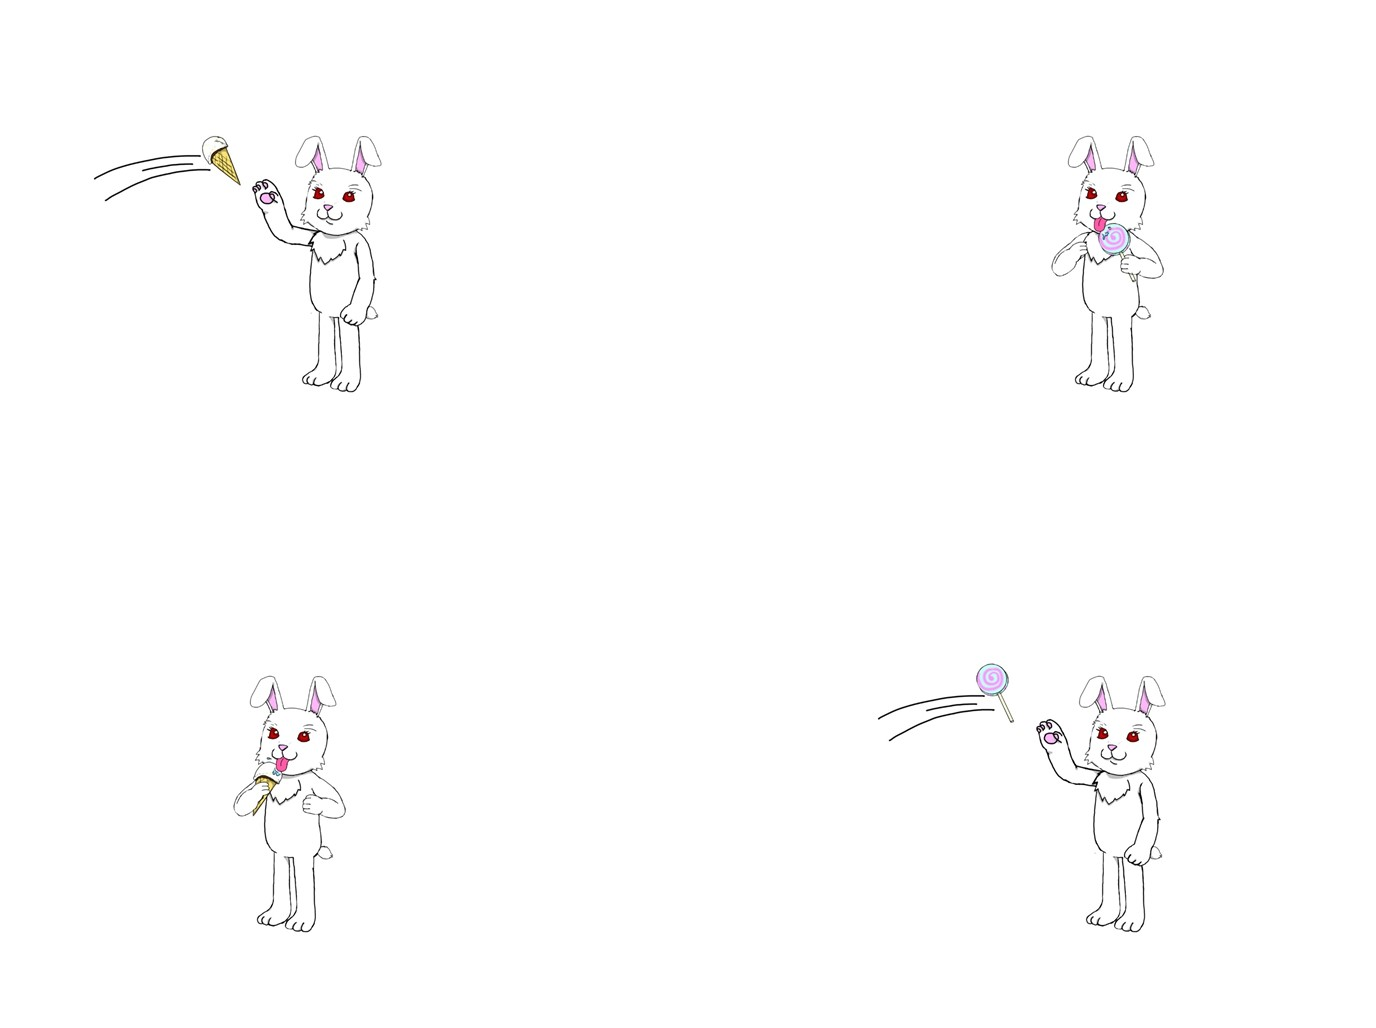
\includegraphics[width=\textwidth,height=\textheight,keepaspectratio]{viz/Fig1-Geetal.jpg}
    \caption{Example 2x2 visual display taken from Ge et al. (2021).}
    \label{fig:sampleslide}
\end{figure}


\subsection{Procedure}

The experiment was hosted on Gorilla \citep{Anwyl-Irvine_2019} and distributed via Prolific, with participants completing the study on a personal computer in an environment that met the experiment’s requirements, such as adequate lighting and minimal background noise. Only participants who consented and passed the hearing and eye-tracking calibration screenings proceeded to the main experiment.

Participants started with the first three tasks in a fixed order: digit span, auditory sensitivity, and Flanker. The digit span task began with two digits. Each digit appeared on screen for 500 ms, followed by a fixation cross for 250 ms. Participants were required to use their mouse to click a visual number pad and enter the same digits in the same order. The adaptive, forward task increased by one digit after each correct response and decreased by one digit after each incorrect response. The task contained 13 trials and took approximately two minutes to complete. The internal consistency of the items as measured by Cronbach's alpha was .63. 

The auditory sensitivity task included four same/different (AX) discrimination tasks across four dimensions or cues:  pitch, risetime (the speed at which a sound reaches its peak amplitude), duration, and formant contrasts. The internal consistency of these tasks, measured by Cronbach’s alpha, was .75, .76, .60, .70, respectively. Each task consisted of 36 trials in which a sound was played, followed by a 250 ms fixation cross, and then a second sound. Participants responded by pressing the ‘Z’ or ‘M’ key to indicate whether the sounds were the same or different. Each task used a continuum of 50 stimuli taken from \citep{Kachlicka_Saito_Tierney_2019}, with 10 stimuli selected at varying distances (15-55) (e.g., 10 Hz or 15 Hz for pitch). The order of stimulus distances and same/different trials was randomized. Each battery task took approximately 90 seconds to complete. We note that both the auditory sensitivity and digit span tasks contained items of varying difficulty. For example, recalling two digits is inherently easier than recalling nine digits; discriminating between two sounds with a 50 Hz difference is easier than discriminating between two sounds with a 5 Hz difference. Given this variability, lower internal reliability, as measured by \cite{Cronbach1951}, is expected. 

The Flanker task showed five arrows with the center arrow facing either the same (congruent) direction as the other four arrows or the opposite (incongruent) direction. Participants were asked to use their keyboard and press ‘Z’ if the middle arrow was facing left and ‘M’ if it was facing right. There were 12 practice trials with feedback followed by 96 trials without feedback (48 congruent; 48 incongruent) spread over four blocks of 24 trials each. After each trial, a fixation cross with varying timing was shown ranging from 400 to 1,000 ms. The internal consistency of the items measured by Cronbach’s alpha was .93.

Next, participants either took part in the main eye-tracking task or the auditory-motor tasks. The eye-tracking task and the auditory-motor tasks were counterbalanced across participants to mitigate order effects and minimize potential biases related to task sequencing. For the eye-tracking task, gaze data were recorded using WebGazer.js \citep{Papoutsaki}, implemented within Gorilla \citep{Anwyl-Irvine_2019}. Participants began with four practice trials followed by 44 experimental trials (20 target and 24 filler). The same two counterbalanced lists used in \cite{Ge2021} were used for the present study. In each trial, the 2x2 visual display and auditory stimulus were presented simultaneously followed by 1,000 ms of silence. Participants were told to simply look at the visual display and listen to the audio. After each trial, a 1,000 ms slide with a different cartoon character at the center of the screen was shown before advancing to the next trial. No feedback was given during the task. The eye-tracking task took approximately 15 minutes to complete.

The auditory-motor tasks consisted of two components: auditory-motor rhythm and auditory-motor melody, both adapted from \citep{Kachlicka_Saito_Tierney_2019}. In the auditory-motor rhythm task, participants heard a rhythmic sequence consisting of 13 possible beat positions, played three times. They were then required to replicate the rhythm by pressing the space bar at the correct intervals. Each key press was time-stamped, and accuracy was assessed based on whether a beat was present (1) or absent (0). In the auditory-motor melody task, participants listened to a seven-note melody and were required to reproduce it using on-screen buttons corresponding to relative pitch levels. To maintain consistency, all melodies began with the middle pitch, ensuring a stable reference point for participants. Accuracy was determined by comparing the selected pitch to the correct response. The internal consistency of the items as measured by Cronbach's alpha was .92.

After completing the eye-tracking task and auditory-motor tasks, the participants completed a modified version of the English LexTALE task \citep{lemhofer2012introducing}. On each trial, participants were shown a fixation cross for 500 ms followed by a string of letters presented for 2000 ms. Participants used the ‘J’ and ‘K’ keys to indicate whether the displayed string was a real word or a non-word, within the given time limit. A total of 60 trials were completed, consisting of 40 words and 20 non-words presented in a randomized order. The internal consistency for the LexTALE task, measured by Cronbach’s alpha, was .92. The English LexTALE and was adapted from publicly available Gorilla open materials; while the original versions of LexTALE did not impose time limits, our version required responses within 2000 ms. The task took approximately three minutes to complete. Lastly, Participants completed a language questionnaire that detailed their language experience. 


\subsection{Data analysis}

Analyses were carried out in R (version 4.4.3; \cite{R}) with a 0.05 alpha level for all null hypothesis significance tests. The individual difference measures were calculated so that each participant had a single score for each task. Working memory capacity was assessed using a digit span task, where participants recalled sequences of numbers in increasing length. Each sequence was scored as correct (1) or incorrect (0), mean sequence length correctly recalled were calculated for each participant. The final working memory score was determined by averaging the correctly recalled sequence lengths. One participant was removed for low performance in this tasks (outside 3 MAD).

For the four auditory sensitivity tasks, all reaction times below 200 ms were removed across the four battery tasks. Following this, hits and false-alarms for each trial were scored and sensitivity to each contrast type (pitch, duration, formants, risetime) was then calculated using d-prime. for all d$'$ calculated measures a constant of .05 was added to both hits/false-alarms with a Haldane correction/log-linear correction for values of 0 or 1 \citep{Hautus1995}. One participant was removed for low performance in these tasks (outside 3 MAD).

The flanker task was analyzed using drift rate estimates from a drift diffusion model (DDM) implemented in the brms package \citep{burkner2017brms}). Reaction times were first filtered to remove extreme responses below 200 ms (anticipatory responses) and above 1750 ms (slow, inattentive responses). Trials were categorized as congruent (flankers match the target) or incongruent (flankers mismatch the target), and reaction time distributions were analyzed separately for each condition. A hierarchical Bayesian DDM was fit to the data using brms, with reaction time as the dependent variable and accuracy as the decision variable. The model was specified with a Wiener diffusion family, estimating key DDM parameters, including drift rate (v), boundary separation (a), non-decision time (t), and bias (z). The primary measure of cognitive control was drift rate (v), reflecting the efficiency of evidence accumulation in resolving response conflict. Individual drift rate estimates were extracted for each participant from the model’s random effects structure. These values were used as the final measure of cognitive control, aligning with prior work that treats drift rate as a sensitivity index for attentional selection in flanker tasks \citep{poole2024spotlight}. 

For both auditory motor tasks scores were computed so that each participant had a single score for each task. In the melody task, each individual note in a trial was scored as 1 for correct and 0 for incorrect, and these values were averaged within each trial to obtain a trial-level accuracy score. The final Melody Score was then calculated as the mean trial accuracy across all trials. Errors were further categorized as sharp (higher than the correct pitch) or flat (lower than the correct pitch). In the rhythm task, each individual beat within a trial was also scored as 1 for correct and 0 for incorrect, with these values averaged within each trial to determine trial accuracy. Reaction times were normalized by subtracting an initial offset to align responses with the expected rhythmic structure. Trials where participants produced double beats (multiple keypresses within a single beat position) were adjusted by retaining only the first response. The final Rhythm Score was calculated as the mean trial accuracy across all trials. Three participants were removed for low performance below three three median absolute deviations in these tasks.

For eye-tracking data removal, eye-fixations outside the possible screen area were removed. As suggested in \cite{bramlett_wiener_24-AOW}, quadrants were defined by the origin to maximize signal retention. Fixations at the beginning of the trials were normally distributed from the center at the beginning trials along both the x and y axes. Eye-fixations with face confirmation below 100\% certainty were removed. We retained approximately 77.79\% of eye-fixations. Our data removal is slightly higher the other recent web-based eye-tracking studies. This is likely do to the fact that we removed data that had less than 100\% face confirmation due to the fact that the task is a look and listen task and we had no other way to ensure that participants were attending to the task. We set a minimal frame rate for participants to 5 fps \citep{Vos_2017} and only five participants were removed.

Like acoustic sensitivity measures, the scores for LexTALE exclude responses with RTs below 200 (ms). While lexTALE is most commonly calculated by averaging the accuracy of non-words and words to control for bias \citep{lemhofer2012introducing}, we calculated LexTALE scores by using d$'$ after ignoring non-responses, which also controls for bias by using the difference between z-scored hits and false-alarms. For all d$'$ calculated measures a constant of .05 was added to both hits/false-alarms with a Haldane (log linear) correction for values of 0 \citep{Hautus1995}. 

For the Language background questionnairre participants first language and dominant langauge were used to confirm their native speaker status \cite{Brown_Tusmagambet_Rahming_Tu_DeSalvo_Wiener_2023}.
Interestingly, 11 particpants had language experience that mismatched their prolific designation (e.g. their primary language they provided in our questionnaire did not match what they self categorized as on prolific). However, the mismatching was not randomly distributed. Of the 11 participants that had mismatched language background information 10 came from the English group and one from the Dutch group. The One dutch speaker self reported English being their dominant language even though their L1 is Dutch.

